 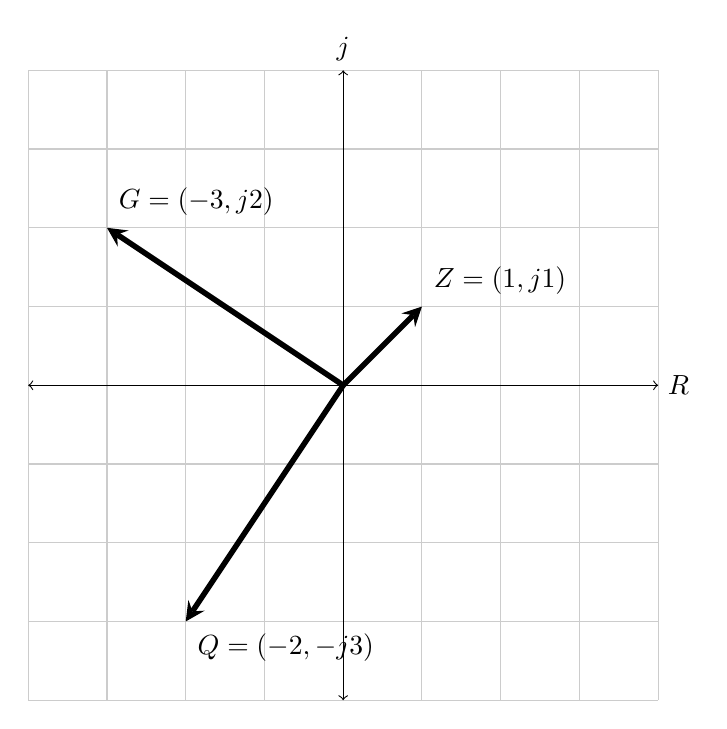
\begin{tikzpicture}
        \draw[thin,gray!40] (-4,-4) grid (4,4);
        \draw[<->] (-4,0)--(4,0) node[right] {$R$};
        \draw[<->] (0,-4)--(0,4) node[above]{$j$};
        \draw[line width=2pt,black,-stealth](0,0)--(1,1) node[anchor=south west]{${Z=(1,j1)}$};
        \draw[line width=2pt,black,-stealth](0,0)--(-3,2) node[anchor=south west]{${G=(-3,j2)}$};
        \draw[line width=2pt,black,-stealth](0,0)--(-2,-3) node[anchor=north west]{${Q=(-2,-j3)}$};
    \end{tikzpicture}
    \caption{Ejemplo de representacion de numero en el plano complejo}